\documentclass[a4paper, 12pt]{article}

\usepackage{fontspec}
\setmainfont{STIX Two Text}
\newfontfamily{\defaultfont}{STIX Two Text}
\newfontfamily{\thaifont}[Scale=MatchLowercase]{TH Sarabun Chula}

\usepackage{polyglossia}
\setdefaultlanguage{thai}
\setotherlanguages{english}

\usepackage[Latin, Thai]{ucharclasses}
\setDefaultTransitions{\defaultfont}{}
\setTransitionTo{Thai}{\thaifont}

\XeTeXlinebreaklocale "th_TH"
\XeTeXlinebreakskip = 0pt plus 1pt

\linespread{1.25}

\usepackage{amsmath, amsthm, amssymb}
\usepackage{unicode-math}
\setmathfont{STIX Two Math}
\usepackage[margin=2cm]{geometry}
\usepackage{siunitx}
\usepackage{chemformula}
\usepackage{fancyhdr}
\usepackage{float}
\usepackage{tcolorbox}

\pagestyle{fancy}
\rhead{Ittipat}
\lhead{รหัสวิชา 49 ฟิสิกส์ \\
วันเสาร์ที่ 19 มีนาคม พ.ศ. 2565}

\begin{document}
\renewcommand{\thefootnote}{\fnsymbol{footnote}}
\renewcommand{\labelenumii}{\theenumii}
\renewcommand{\theenumii}{\arabic{enumii}.}
\renewcommand{\arraystretch}{1.5}
กำหนดให้ใช้ค่าต่อไปนี้ สำหรับกรณีที่ต้องแทนค่าตัวเลข
\begin{itemize}
    \item[] ความเร่งโน้มถ่วง \(g=\SI{9.8}{m/s^2}\)
    \item[] อัตราเร็วของแสงในสุญญากาศ \(c=\SI{3.0e8}{m/s}\)
    \item[] ค่าคงตัวแก๊ส \(R=\SI{8.3}{J/(mol\,K)}\)
    \item[] ค่าคงตัวอโวกาโดร \(N_\text{A}=\SI{6.0e23}{mol^{-1}}\)
    \item[] ค่าคงตัวโบลต์ซมันน์ \(k_\text{B}=\SI{1.4e-23}{J/K}\)
    \item[] ค่าของ \(\sin\theta\;\cos\theta\) และ \(\tan\theta\) ที่มีมุม \(\theta\) ต่าง ๆ ดังตารางต่อไปนี้
\end{itemize}
\begin{table}[H]
    \centering
    \begin{tabular}{|c|c|c|c|c|c|}
        \hline
        \(\theta\)     & \SI{0}{\degree} & \SI{30}{\degree}       & \SI{45}{\degree}       & \SI{60}{\degree}       & \SI{90}{\degree} \\
        \hline
        \(\sin\theta\) & \(0\)           & \(\frac{1}{2}\)        & \(\frac{\sqrt{2}}{2}\) & \(\frac{\sqrt{3}}{2}\) & 1                \\
        \hline
        \(\cos\theta\) & \(1\)           & \(\frac{\sqrt{3}}{2}\) & \(\frac{\sqrt{2}}{2}\) & \(\frac{1}{2}\)        & \(0\)            \\
        \hline
        \(\tan\theta\) & \(0\)           & \(\frac{1}{\sqrt{3}}\) & \(1\)                  & \(\sqrt{3}\)           & ไม่นิยาม           \\
        \hline
    \end{tabular}
\end{table}
\begin{tcolorbox}[
        box align=center,
        halign=flush center,
        valign=center
    ]
    ข้อสอบฉบับนี้อ้างอิงจากข้อสอบ \textbf{ฟิสิกส์ วิชาสามัญ พ.ศ. 2565 ชุดที่ 1} \\
    หากพบปัญหาหรือต้องการสอบถาม ติดต่อ ittipatken@gmail.com
\end{tcolorbox}
\newpage
\begin{enumerate}
    \item วัดขนาดของวัตถุปริซึมสี่เหลี่ยมที่มีฐานเป็นรูปสี่เหลี่ยมจัตุรัส ดังภาพ \\
          \begin{figure}[H]
              \centering
              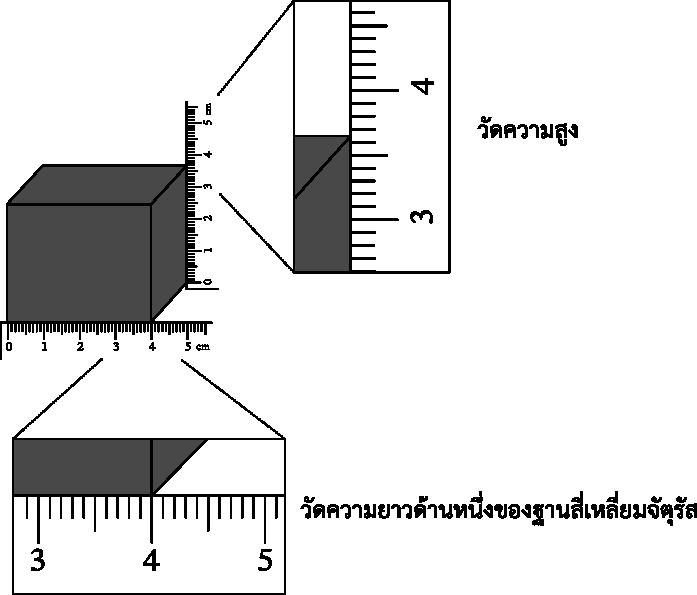
\includegraphics{images/5_1.pdf}
          \end{figure}
          ปริซึมนี้มีปริมาตรกี่ลูกบาศก์เซนติเมตร โดยคำนึงถึงเลขนัยสำคัญ \\
          กำหนดให้ อ่านค่าความสูงและความยาวจากภาพที่ขยายเท่านั้น
          \begin{enumerate}
              \item 53.29
              \item 53.3
              \item 58
              \item 58.4
              \item 58.40
          \end{enumerate}
          \newpage
    \item เจ้าหน้าที่กู้ภัยต้องการโยนอุปกรณ์ให้คนที่อยู่ในตึกซึ่งอยู่ห่าง \(5\) เมตร และอยู่สูง \(\dfrac{5\sqrt{3}}{2}\) เมตร ดังภาพ \\
          กำหนดให้ ไม่คิดแรงต้านอากาศ \\
          \begin{figure}[H]
              \centering
              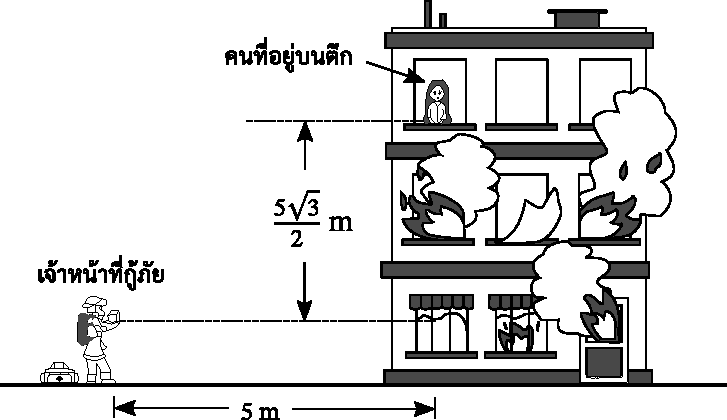
\includegraphics{images/2_2.pdf}
          \end{figure}
          เจ้าหน้าที่กู้ภัยต้องโยนอุปกรณ์ด้วยมุมกี่องศาเทียบกับแนวระดับ เพื่อให้อุปกรณ์ขณะรับมีความความเร็วในแนวดิ่งเป็นศูนย์
          \begin{enumerate}
              \item 30
              \item 37
              \item 45
              \item 53
              \item 60
          \end{enumerate}
          \newpage
    \item ลูกกลมมวล \(m_1\) มีมวลเป็นครึ่งหนึ่งของ \(m_2\) ถูกผูกด้วยเชือกที่ยาวไม่เท่ากันไว้ที่จุดตรึงหนึ่ง เมื่อแกว่งลูกกลมทั้งสองลูกให้เริ่มเคลื่อนที่พร้อมกันเป็นวงกลมในระนาบเดียวกันและมีจุดศูนย์กลางร่วมกัน พบว่ารัศมีการเคลื่อนที่ของลูกกลม \(m_2\) มีค่าเป็นสองเท่าของรัศมีการเคลื่อนที่ของลูกกลม \(m_1\) ดังภาพ \\
          \begin{figure}[H]
              \centering
              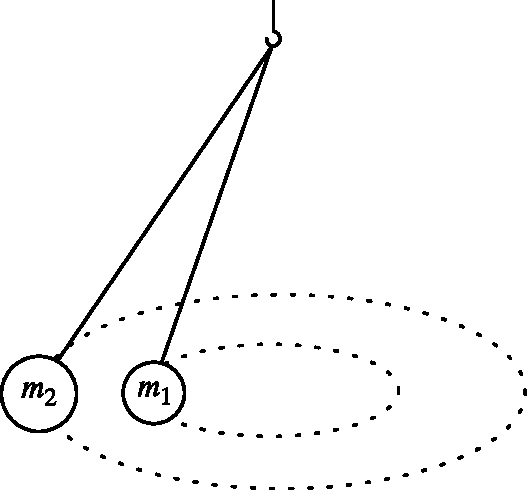
\includegraphics[scale = 0.8]{images/3_3.pdf}
          \end{figure}
          ข้อใดถูกต้อง
          \begin{enumerate}
              \item คาบของ \(m_1\) มีค่าน้อยกว่าคาบของ \(m_2\)
              \item ความถี่เชิงมุมของ \(m_1\) มีค่าน้อยกว่าความถี่เชิงมุมของ \(m_2\)
              \item อัตราเร็วเชิงมุมของ \(m_1\) มีค่าเท่ากับอัตราเร็วเชิงมุมของ \(m_2\)
              \item อัตราเร็วเชิงเส้นของ \(m_1\) มีค่าเท่ากับอัตราเร็วเชิงเส้นของ \(m_2\)
              \item แรงสู่ศูนย์กลางของ \(m_1\) มีค่ามากกว่าแรงสู่ศูนย์กลางของ \(m_2\)
          \end{enumerate}
          \newpage
    \item แกว่งลูกตุ้มมวล \(m\) ที่ผูกเชือกยาว \(L\) ให้เคลื่อนที่แบบฮาร์มอนิกอย่างง่ายระหว่างจุด A และจุด B ดังภาพ พบว่าลูกตุ้มแกว่งครบ \(10\) รอบ ใช้เวลา \(2\pi\) วินาที
          \begin{figure}[H]
              \begin{minipage}[ht]{0.75\linewidth}
                  พิจารณาข้อความต่อไปนี้
                  \begin{itemize}
                      \item[ก.] ที่จุด A และ B ขนาดของความเร็วมีค่าเท่ากันและไม่เท่ากับศูนย์
                      \item[ข.] เมื่อแกว่งลูกตุ้มมวล \(m\) ที่ผูกเชือกยาว \(L\) คาบการแกว่ง เท่ากับ \(0.2\pi\)
                      \item[ค.] เมื่อแกว่งลูกตุ้มมวล \(2m\) ที่ผูกเชือกยาว \(L\) ความถี่เชิงมุมมากกว่าเมื่อแกว่งลูกตุ้มมวล \(m\) ที่ผูกเชือกยาว \(2L\) วินาที
                  \end{itemize}
              \end{minipage}
              \begin{minipage}[ht]{0.2\linewidth}
                  \begin{figure}[H]
                      \raggedleft
                      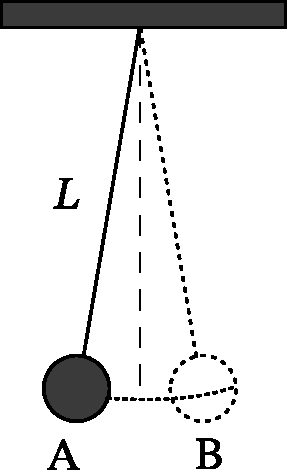
\includegraphics[scale = 0.6]{images/4_4.pdf}
                  \end{figure}
              \end{minipage}
          \end{figure}
          \begin{enumerate}
              \item ก. เท่านั้น
              \item ข. เท่านั้น
              \item ค. เท่านั้น
              \item ก. และ ข.
              \item ข. และ ค.
          \end{enumerate}
          \newpage
    \item รถบรรทุกมวล \(M\) ขนตู้มวล \(m\) บนกระบะ เคลื่อนที่ด้วยความเร็วต้น \(\vec{u}\) ดังภาพ \\
          \begin{tabular}{rl}
              กำหนดให้ & \(\mu_k\) เป็นสัมประสิทธิ์ความเสียดทานจลน์ระหว่างตู้และพื้นกระบะรถบรรทุก \\
                     & \(\mu_s\) เป็นสัมประสิทธิ์ความเสียดทานสถิตระหว่างตู้และพื้นกระบะรถบรรทุก \\
                     & \(g\) เป็นขนาดของความเร่งโน้มถ่วง
          \end{tabular}
          \begin{figure}[H]
              \centering
              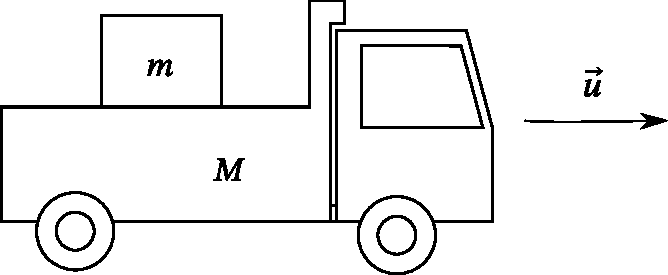
\includegraphics[scale = 0.9]{images/6_5.pdf}
          \end{figure}
          ถ้าต้องการให้รถหยุดนิ่งโดยที่ตู้ยังอยู่นิ่งเทียบกับรถ ระยะทางที่สั้นที่สุดตั้งแต่เริ่มเบรกจนกระทั่งรถหยุดนิ่งเป็นเท่าใด
          \begin{enumerate}
              \item \(\dfrac{u^2}{2\mu_s g}\)
              \item \(\dfrac{u^2}{2\mu_k g}\)
              \item \(\dfrac{u^2}{(\mu_k+\mu_s) g}\)
              \item \(\left(\dfrac{M+m}{m}\right)\dfrac{u^2}{2\mu_s g}\)
              \item \(\left(\dfrac{M+m}{m}\right)\dfrac{u^2}{2\mu_k g}\)
          \end{enumerate}
          \newpage
    \item กระถางต้นไม้มวล \(m\) ถูกแขวนอยู่บนเส้นลวดสองเส้นคือ A และ B ซึ่งยึดติดกับเสาสองต้น โดยมุมที่เส้นลวด A กระทำกับเส้นแนวระดับเท่ากับ \(\theta\) และเส้นลวด A และ B ทำมุมกัน \(90\) องศา ดังภาพ \\
          กำหนดให้ \(g\) เป็นขนาดของความเร่งโน้มถ่วง \\
          \begin{figure}[H]
              \centering
              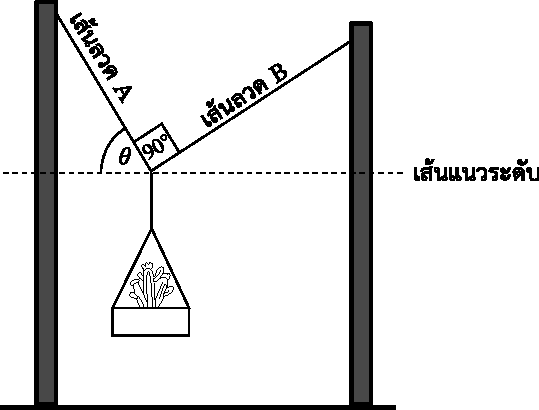
\includegraphics{images/7_6.pdf}
          \end{figure}
          ขนาดของแรงดึงในเส้นลวด B มีค่าเท่าใด
          \begin{enumerate}
              \item \(mg\sin\theta\)
              \item \(mg\cos\theta\)
              \item \(mg\tan\theta\)
              \item \(\dfrac{mg}{\sin\theta}\)
              \item \(\dfrac{mg}{\tan\theta}\)
          \end{enumerate}
          \newpage
    \item ออกแรงกระทำต่อวัตถุ 2 ครั้ง ได้กราฟความสัมพันธ์ระหว่างขนาดของแรง \(F\) ที่กระทำต่อวัตถุกับเวลา \(t\) ดังภาพ \\
          กำหนดให้ ขณะที่วัตถุถูกแรงกระทำ มวลของวัตถุและทิศทางของแรงไม่เปลี่ยนแปลง \\
          \begin{figure}[H]
              \centering
              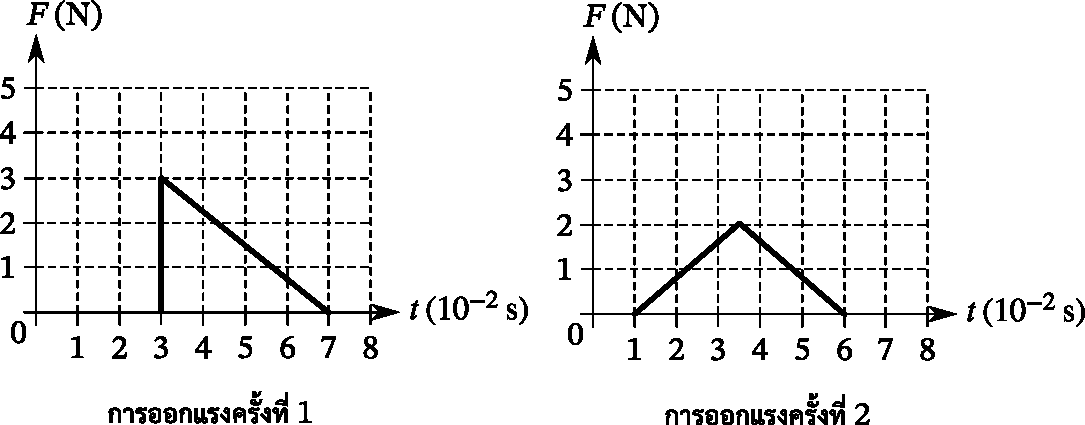
\includegraphics[scale = 0.9]{images/1_7.pdf}
          \end{figure}
          ข้อใดเปรียบเทียบขนาดของการดลครั้งที่ 1 (\(I_1\)) และครั้งที่ 2 (\(I_2\)) ได้ถูกต้อง
          \begin{enumerate}
              \item \(I_1\) มากกว่า \(I_2\) เพราะพื้นที่ใต้กราฟของครั้งที่ 1 มากกว่าครั้งที่ 2
              \item \(I_1\) มากกว่า \(I_2\) เพราะขนาดของแรงสูงสุดของครั้งที่ 1 มากกว่าของครั้งที่ 2
              \item \(I_2\) มากกว่า \(I_1\) เพราะแรงเฉลี่ยของครั้งที่ 2 มากกว่าครั้งที่ 1
              \item \(I_2\) มากกว่า \(I_1\) เพราะช่วงเวลาที่วัตถุถูกแรงกระทำของครั้งที่ 2 มากกว่าของครั้งที่ 1
              \item \(I_2\) มากกว่า \(I_1\) เพราะขนาดของแรงของครั้งที่ 2 ลดลงจากจุดสูงสุดเร็วกว่าของครั้งที่ 1
          \end{enumerate}
          \newpage
    \item คลื่นกลเคลื่อนที่ด้วยอัตราเร็ว \(2.0\) เมตรต่อวินาที เมื่อพิจารณาอนุภาคหนึ่งที่ตำแหน่งใดตำแหน่งหนึ่งในตัวกลาง พบว่า ความสัมพันธ์ระหว่างการกระจัดกับเวลาเป็นดังกราฟ \\
          \begin{figure}[H]
              \centering
              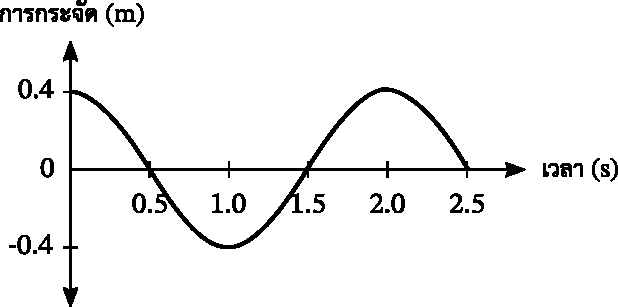
\includegraphics{images/20_8.pdf}
          \end{figure}
          ณ เวลาหนึ่ง ๆ อนุภาคสองอนุภาคใด ๆ ในตัวกลาง ที่มีเฟสต่างกัน \(\dfrac{\pi}{4}\) เรเดียน จะอยู่ห่างกันกี่เมตร
          \begin{enumerate}
              \item 0.1
              \item 0.125
              \item 0.25
              \item 0.5
              \item 1.0
          \end{enumerate}
          \newpage
    \item ปลายเชือกด้านซ้ายของเชือกเส้นหนึ่งถูกตรึงอยู่กับที่ เมื่อสะบัดปลายเชือกด้านขวาทำให้เกิดคลื่นในเส้นเชือก 2 คลื่น ที่มีรูปร่างต่างกัน เคลื่อนที่ในทิศทางเดียวกันด้วยอัตราเร็วเท่ากัน \(1\) เมตรต่อวินาที รูปร่างคลื่น ณ เวลาหนึ่งเป็นดังภาพ \\
          \begin{figure}[H]
              \centering
              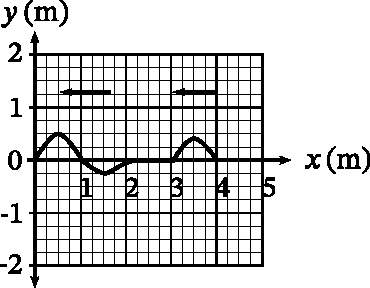
\includegraphics{images/21_9_0.pdf}
          \end{figure}
          ข้อใดแสดงรูปร่างของคลื่นเมื่อเวลาผ่านไป 2 วินาที ได้ถูกต้อง
          \begin{enumerate}
              \item \hfill
                    \begin{figure}[H]
                        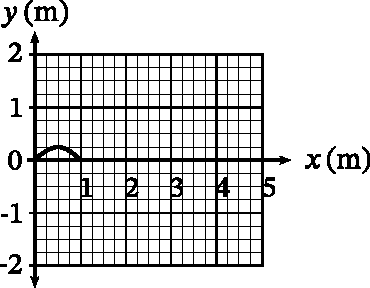
\includegraphics{images/21_9_1.pdf}
                    \end{figure}
              \item \hfill
                    \begin{figure}[H]
                        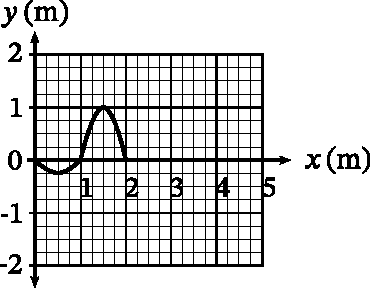
\includegraphics{images/21_9_2.pdf}
                    \end{figure}
                    \vfill
              \item \hfill
                    \begin{figure}[H]
                        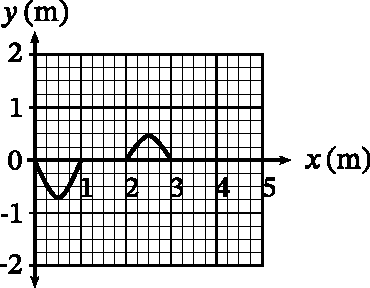
\includegraphics{images/21_9_3.pdf}
                    \end{figure}
              \item \hfill
                    \begin{figure}[H]
                        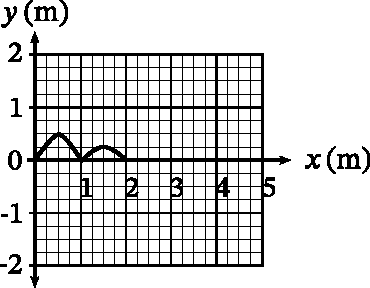
\includegraphics{images/21_9_4.pdf}
                    \end{figure}
              \item \hfill
                    \begin{figure}[H]
                        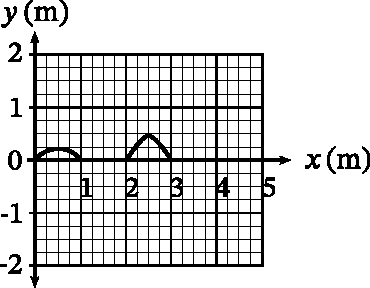
\includegraphics{images/21_9_5.pdf}
                    \end{figure}
          \end{enumerate}
          \newpage
    \item ในการเตรียมงานจุดพลุใกล้ชุมชนหนึ่ง ผู้จัดงานทำการตรวจสอบระดับเสียง โดยทดสอบจุดพลุที่ทำให้เกิดเสียงที่มีความถี่ประมาณ \(1000\) เฮิรตซ์ ในสถานที่เตรียมจัดงาน พบว่า ที่ระยะห่างจากจุดที่ทดสอบ \(15\) เมตร วัดระดับเสียงได้ \(140\) เดซิเบล \\
          \begin{figure}[H]
              \centering
              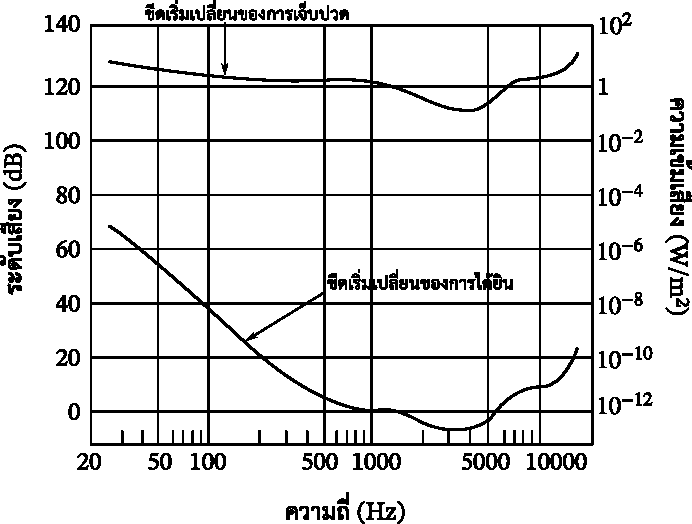
\includegraphics{images/22_10.pdf}
          \end{figure}
          กำหนดให้ ความสัมพันธ์ระหว่างระดับเสียงและความเข้มเสียง กับความถี่ที่คนในชุมชนนี้ได้ยิน เป็นดังกราฟ \\
          จากผลการทดสอบและกราฟข้างต้น บริเวณที่จุดพลุควรอยู่ห่างจากชุมชนอย่างน้อยที่สุดกี่เมตร คนในชุมชนจึงได้ยินเสียงที่ระดับเสียงไม่เกินขีดเริ่มเปลี่ยนของการเจ็บปวด
          \begin{enumerate}
              \item \(1.3\times10\)
              \item \(\num{1.3e2}\)
              \item \(\num{1.5e2}\)
              \item \(\num{1.5e3}\)
              \item \(\num{1.5e8}\)
          \end{enumerate}
          \newpage
    \item นักเรียนศึกษาการบีตของเสียงระหว่างแหล่งกำเนิดเสียงหนึ่งที่มีความถี่ 435 เฮิรตซ์ กับส้อมเสียง 4 อันที่มีความถี่ของเสียง ดังตาราง
          \begin{figure}[H]
              \centering
              \begin{tabular}{|c|c|}
                  \hline
                  ส้อมเสียง & ความถี่ (เฮิรตซ์) \\
                  \hline
                  A       & 425           \\
                  \hline
                  B       & 430           \\
                  \hline
                  C       & 440           \\
                  \hline
                  D       & 445           \\
                  \hline
              \end{tabular}
          \end{figure}
          ถ้าต้องการให้เกิดบีตระหว่างเสียงจากแหล่งกำเนิดเสียงกับเสียงจากการเคาะส้อมเสียง 1 อัน โดยมีความถี่บีตเท่ากับ \(5\) เฮิรตซ์ ควรเลือกใช้ส้อมเสียงใด และเสียงดังกล่าวจะมีเสียงดังเป็นจังหวะกี่ครั้งใน \(2\) วินาที
          \begin{enumerate}
              \item ส้อมเสียง A และ 5 ครั้ง
              \item ส้อมเสียง B และ 5 ครั้ง
              \item ส้อมเสียง C และ 10 ครั้ง
              \item ส้อมเสียง D และ 5 ครั้ง
              \item ส้อมเสียง D และ 10 ครั้ง
          \end{enumerate}
          \newpage
    \item เมื่อฉายแสงเลเซอร์เข้าสู่แท่งพลาสติกรูปครึ่งวงกลมตามแนวรัศมี แสงเลเซอร์ที่ออกจากด้านระนาบจะมีมุมวิกฤตมีค่าเท่ากับ \(30\) องศา ดังภาพ \\
          \begin{figure}[H]
              \centering
              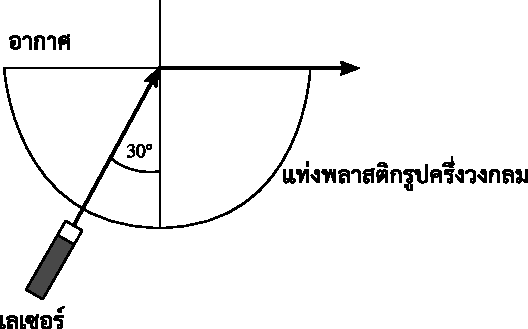
\includegraphics{images/25_12.pdf}
          \end{figure}
          กำหนดให้ อัตราเร็วของแสงในอากาศมีค่าเท่ากับ \(\num{3.0e8}\) เมตรต่อวินาที \\
          ค่าดรรชนีหักเหของอากาศมีค่าเท่ากับ \(1\) \\
          อัตราเร็วของแสงในแท่งพลาสติกจะมีค่ากี่เมตรต่อวินาที และถ้าให้แสงเลเซอร์เดิมเคลื่อนที่จากแท่งพลาสติกไปยังอากาศ ด้วยมุมตกกระทบน้อยลงเป็น \(20\) องศา แสงจะเคลื่อนที่อย่างไร
          \begin{enumerate}
              \item \(\num{1.5e8}\) เมตรต่อวินาที และ แสงจะหักเหออกสู่อากาศด้วยมุมหักเหที่น้อยกว่า \(20\) องศา
              \item \(\num{1.5e8}\) เมตรต่อวินาที และ แสงจะหักเหออกสู่อากาศด้วยมุมหักเหที่มากกว่า \(20\) องศา
              \item \(\num{1.5e8}\) เมตรต่อวินาที และ แสงจะสะท้อนกลับหมดโดยไม่ออกจากตัวกลาง
              \item \(\num{3.0e8}\) เมตรต่อวินาที และ แสงจะหักเหออกสู่อากาศด้วยมุมหักเหที่มากกว่า \(20\) องศา
              \item \(\num{3.0e8}\) เมตรต่อวินาที และ แสงจะสะท้อนกลับหมดโดยไม่ออกจากตัวกลาง
          \end{enumerate}
          \newpage
    \item ฉายแสงเลเซอร์ความยาวคลื่น \(650\) นาโนเมตร ตกกระทบตั้งฉากกับเกรตติง พบว่า เกิดจุดสว่างกลางและจุดสว่างอันดับที่ 1 ที่ตำแหน่งบนฉากซึ่งอยู่ห่างจากเกรตติง \(1.0\) เมตร ดังภาพ \\
          \begin{figure}[H]
              \centering
              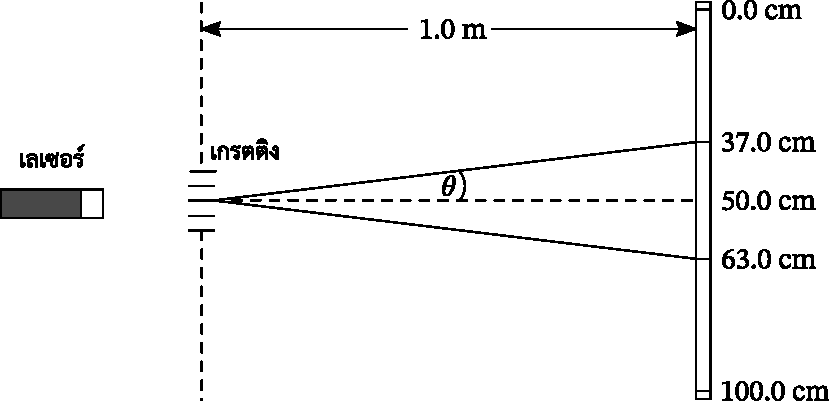
\includegraphics{images/24_13.pdf}
          \end{figure}
          พิจารณาข้อความต่อไปนี้
          \begin{itemize}
              \item[ก.] ระยะห่างระหว่างช่องของเกรตติงมีค่าเท่ากับ \(5.0\) ไมโครเมตร
              \item[ข.] ถ้าฉายแสงเลเซอร์ที่มีความยาวคลื่นน้อยกว่า \(650\) นาโนเมตร ระยะห่างระหว่างจุดสว่างจะมีค่าเพิ่มขึ้น
              \item[ค.] ถ้าใช้เกรตติงอันใหม่ แล้วพบว่าระยะห่างระหว่างจุดสว่างมีค่าน้อยลง แสดงว่าระยะห่างระหว่างช่องของเกรตติงจะมีค่ามากกว่าเดิม
          \end{itemize}
          \begin{enumerate}
              \item ก. เท่านั้น
              \item ข. เท่านั้น
              \item ค. เท่านั้น
              \item ก. และ ค.
              \item ข. และ ค.
          \end{enumerate}
          \newpage
    \item ลวดโลหะ A และ B มีพื้นที่หน้าตัด \(10.0\) และ \(2.0\) ตารางมิลลิเมตร ตามลำดับ \\
          กำหนดให้ ความสัมพันธ์ระหว่างความเค้น (\(\sigma\)) และความเครียด (\(\varepsilon\)) ของลวดโลหะทั้งสองเป็นดังกราฟ \\
          \begin{figure}[H]
              \centering
              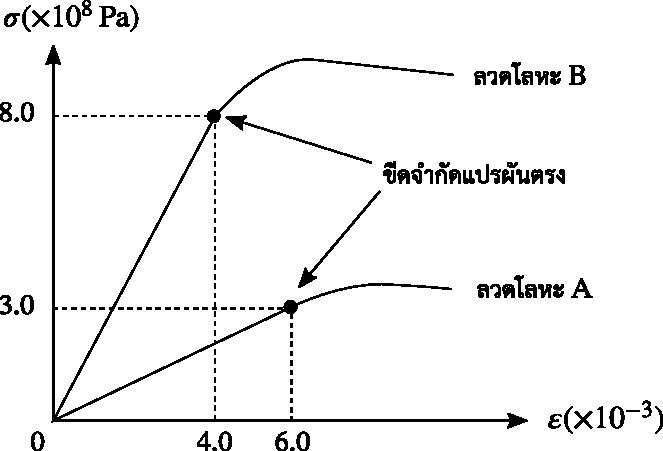
\includegraphics{images/16_14.pdf}
          \end{figure}
          หากต้องการลวดโลหะที่ทนต่อแรงภายนอกที่มากระทำได้มากกว่า โดยยังสามารถกลับมามีความยาวเท่าเดิมควรเลือกลวดโลหะใด และมอดุลัสของยังของลวดโลหะดังกล่าวมีค่ากี่พาสคัล
          \begin{enumerate}
              \item ลวดโลหะ A และ \num{2.0e-11} พาสคัล
              \item ลวดโลหะ A และ \num{5.0e10} พาสคัล
              \item ลวดโลหะ B และ \num{5.0e-12} พาสคัล
              \item ลวดโลหะ B และ \num{8.0e8} พาสคัล
              \item ลวดโลหะ B และ \num{2.0e11} พาสคัล
          \end{enumerate}
          \newpage
    \item ทรงกระบอกที่มีลูกสูบเคลื่อนที่ได้คล่อง ภายในบรรจุแก๊สอุดมคติ \(2\) โมล อุณหภูมิ \(67\) องศาเซลเซียสและมีความดันคงตัวเท่ากับ \(10\) กิโลพาสคัล \\
          กำหนดให้ \(R\) เป็นค่าคงตัวแก๊ส \\
          ถ้าลดอุณหภูมิของแก๊สลงช้า ๆ จนเหลือ \(48\) องศาเซลเซียส โดยความดันเท่าเดิม งานที่เกิดขึ้นเมื่อลูกสูบเคลื่อนที่มีค่าเท่าใด และระบบมีการเปลี่ยนแปลงปริมาตรอย่างไร
          \begin{enumerate}
              \item \(3.8R\times10^{-3}\) และ ปริมาตรลดลง
              \item \(38R\) และ ปริมาตรลดลง
              \item \(38R\) และ ปริมาตรเพิ่มขึ้น
              \item \(3.8R\times10^5\) และ ปริมาตรลดลง
              \item \(3.8R\times10^5\) และ ปริมาตรเพิ่มขึ้น
          \end{enumerate}
          \newpage
    \item ดัดลวดขนาดเล็กมาก มวล \(2.0\) กรัม ให้เป็นวงรูปสี่เหลี่ยมผืนผ้า กว้าง \(2.4\) เซนติเมตร ยาว \(2.5\) เซนติเมตร แล้วผูกด้วยเชือกเบาและนำไปวางบนผิวของของเหลวชนิดหนึ่งที่มีความตึงผิว \(0.4\) นิวตันต่อเมตร จากนั้นออกแรงดึงเชือก ดังภาพ \\
          \begin{figure}[H]
              \centering
              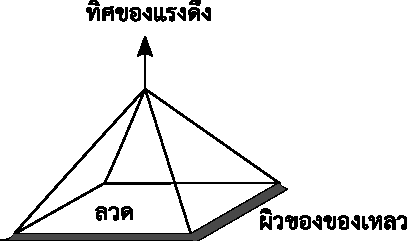
\includegraphics{images/15_16.pdf}
          \end{figure}
          ถ้าต้องการให้ลวดหลุดออกจากผิวของของเหลวได้ จะต้องออกแรงดึงขนาดอย่างน้อยกี่นิวตัน
          \begin{enumerate}
              \item \num{3.9e-2}
              \item \num{4.9e-2}
              \item \num{5.9e-2}
              \item \num{7.8e-2}
              \item \num{9.8e-2}
          \end{enumerate}
          \newpage
    \item ตัวนำทรงกลม A และ B มีมวล \(M\) เท่ากัน แต่ขนาดประจุไฟฟ้าบนตัวนำทรงกลม A เท่ากับ \(Q\) ส่วนตัวนำทรงกลม B มีขนาดประจุไฟฟ้าเป็น \(n\) เท่าของตัวนำทรงกลม A \\
          \begin{figure}[H]
              \begin{minipage}[ht]{0.45\linewidth}
                  วางตัวนำทรงกลม A ไว้บนพื้นที่เป็นฉนวน แล้วนำตัวนำทรงกลม B ที่ผูกด้วยเชือกเบาเข้าใกล้ตัวนำทรงกลม A ในแนวดิ่ง โดยให้ระยะห่างระหว่างจุดศูนย์กลางของตัวนำทรงกลมทั้งสอง เท่ากับ \(d\) ดังภาพ \\

                  \begin{tabular}{rl}
                      กำหนดให้ & \(k\) เป็นค่าคงตัวคูลอมบ์          \\
                             & \(g\) เป็นขนาดของความเร่งโน้มถ่วง \\
                  \end{tabular}
              \end{minipage}
              \begin{minipage}[ht]{0.5\linewidth}
                  \begin{figure}[H]
                      \raggedleft
                      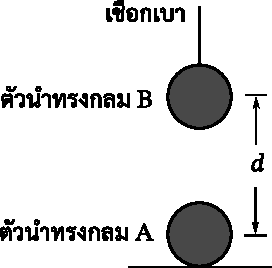
\includegraphics{images/8_17.pdf}
                  \end{figure}
              \end{minipage}
          \end{figure}
          ถ้าต้องการให้ตัวนำทรงกลม A เริ่มจะลอยขึ้นจากพื้นได้ ชนิดประจุไฟฟ้าบนตัวนำทรงกลมทั้งสองจะต้องเป็นอย่างไร และระยะห่าง \(d\) จะต้องมีค่ามากที่สุดเท่าใด
          \begin{figure}[H]
              \centering
              \begin{tabular}{c|c|c|}
                  \cline{2-3}
                     & ชนิดประจุไฟฟ้า & ระยะห่าง \(d\)              \\
                  \cline{2-3}
                  1. & ชนิดเดียวกัน   & \(\sqrt{\dfrac{nkQ}{Mg}}\) \\
                  \cline{2-3}
                  2. & ชนิดเดียวกัน   & \(Q\sqrt{\dfrac{k}{Mg}}\)  \\
                  \cline{2-3}
                  3. & ชนิดต่างกัน    & \(\sqrt{\dfrac{nkQ}{Mg}}\) \\
                  \cline{2-3}
                  4. & ชนิดต่างกัน    & \(Q\sqrt{\dfrac{k}{Mg}}\)  \\
                  \cline{2-3}
                  5. & ชนิดต่างกัน    & \(Q\sqrt{\dfrac{nk}{Mg}}\) \\
                  \cline{2-3}
              \end{tabular}
          \end{figure}
          \newpage
    \item เครื่องดักจับฝุ่นด้วยไฟฟ้าสถิตชนิดหนึ่งมีหลักการทำงาน โดยให้อากาศที่มีอนุภาคฝุ่นเคลื่อนที่ผ่านส่วนที่สร้างประจุไฟฟ้า เพื่อให้อนุภาคฝุ่นมีประจุไฟฟ้าลบ แล้วเคลื่อนที่ไปยังแผ่นรับฝุ่นที่มีขั้วไฟฟ้า \\
          พิจารณาอนุภาคฝุ่น A และ B ซึ่งอนุภาคฝุ่น A มีมวลมากกว่า B และอัตราส่วนระหว่างประจุต่อมวลของ A มากกว่าของ B ขณะอนุภาคทั้งสองเคลื่อนที่เข้าหาแผ่นรับฝุ่น ดังภาพ \\
          \begin{figure}[H]
              \centering
              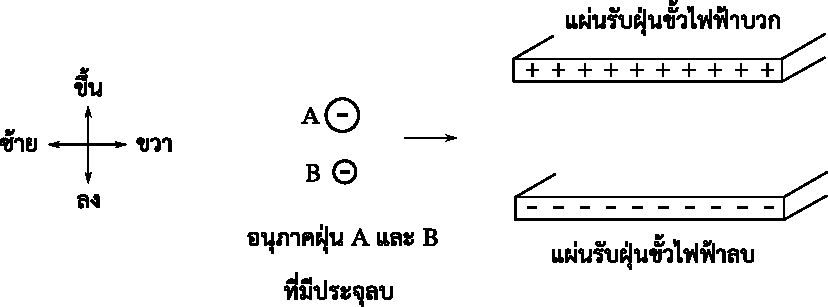
\includegraphics{images/9_18.pdf}
          \end{figure}
          กำหนดให้ แรงโน้มถ่วงมีขนาดน้อยมากเมื่อเทียบกับแรงเนื่องจากสนามไฟฟ้าระหว่างแผ่นรับฝุ่น \\
          สนามไฟฟ้าระหว่างแผ่นรับฝุ่นมีทิศทางใด และขณะอนุภาคฝุ่นทั้งสองเคลื่อนที่ในสนามไฟฟ้า ขนาดของความเร่งและขนาดประจุเป็นไปตามข้อใด
          \begin{figure}[H]
              \centering
              \begin{tabular}{c|c|c|c|}
                  \cline{2-4}
                     & ทิศทางของสนามไฟฟ้า & ขนาดความเร่ง & ขนาดประจุ   \\
                  \cline{2-4}
                  1. & ขึ้น               & A น้อยกว่า B  & A น้อยกว่า B \\
                  \cline{2-4}
                  2. & ขึ้น               & A มากกว่า B  & A มากกว่า B \\
                  \cline{2-4}
                  3. & ลง               & A น้อยกว่า B  & A น้อยกว่า B \\
                  \cline{2-4}
                  4. & ลง               & A เท่ากับ B   & A มากกว่า B \\
                  \cline{2-4}
                  5. & ลง               & A มากกว่า B  & A มากกว่า B \\
                  \cline{2-4}
              \end{tabular}
          \end{figure}
          \newpage
    \item แบตเตอรี่ขนาด \(12\) โวลต์ ที่มีความต้านทานภายใน \(1\) โอห์ม ต่ออยู่กับอุปกรณ์ไฟฟ้าที่มีความต้านทาน \(R_1 = \SI{10}{\ohm}\) และตัวต้านทานที่มีความต้านทาน \(R_2 = \SI{10}{\ohm}\) ดังภาพ \\
          \begin{figure}[H]
              \centering
              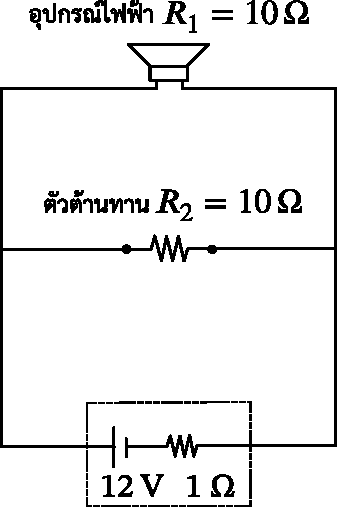
\includegraphics{images/11_19.pdf}
          \end{figure}
          พลังงานไฟฟ้าที่อุปกรณ์ไฟฟ้าใช้ไปใน 30 วินาที มีค่ากี่จูล
          \begin{enumerate}
              \item 12
              \item 300
              \item 432
              \item 600
              \item 1200
          \end{enumerate}
          \newpage
    \item ณ อุณหภูมิหนึ่ง ลวดตัวนำ A B และ C มีความยาวและความต้านทาน ดังตาราง \\
          \begin{figure}[H]
              \centering
              \begin{tabular}{|c|c|c|}
                  \hline
                  ลวดตัวนำ & ความยาว (เมตร) & ความต้านทาน (โอห์ม) \\
                  \hline
                  A      & 1.0            & 2.2               \\
                  \hline
                  B      & 2.0            & 4.4               \\
                  \hline
                  C      & 2.0            & 5.2               \\
                  \hline
              \end{tabular}
          \end{figure}
          พิจารณาข้อความต่อไปนี้
          \begin{itemize}
              \item[ก.] ถ้าลวดตัวนำ A มีสภาพต้านทานไฟฟ้า \num{2.2e-7} โอห์ม เมตร จะมีพื้นที่หน้าตัด 0.1 ตารางมิลลิเมตร
              \item[ข.] ถ้าลวดตัวนำ A และ B มีสภาพต้านทานไฟฟ้าเท่ากัน พื้นที่หน้าตัดของลวดตัวนำ A จะมากกว่า B
              \item[ค.] ถ้าลวดตัวนำ C มีความยาว 1.0 เมตร โดยพื้นที่หน้าตัดเท่าเดิม จะมีความต้านทาน 10.4 โอห์ม
          \end{itemize}
          ข้อความใดถูกต้อง
          \begin{enumerate}
              \item ก. เท่านั้น
              \item ข. เท่านั้น
              \item ก. และ ค. เท่านั้น
              \item ข. และ ค. เท่านั้น
              \item ก. ข. และ ค.
          \end{enumerate}
          \newpage
    \item ขดลวดรูปสี่เหลี่ยมผืนผ้ามีพื้นที่ \(0.50\) ตารางเมตร อยู่ในบริเวณที่มีสนามแม่เหล็กสม่ำเสมอ \(\vec{B}\) ในทิศ \(+z\) \\
          ในขณะเริ่มต้น ระนาบของขดลวดวางตัวอยู่ในระนาบ \(xy\) จากนั้นหมุนขดลวดรอบแกน \(y\) โดยระนาบของขดลวดทำมุม \(\theta\) กับระนาบ \(xy\) ดังภาพ \\
          \begin{figure}[H]
              \centering
              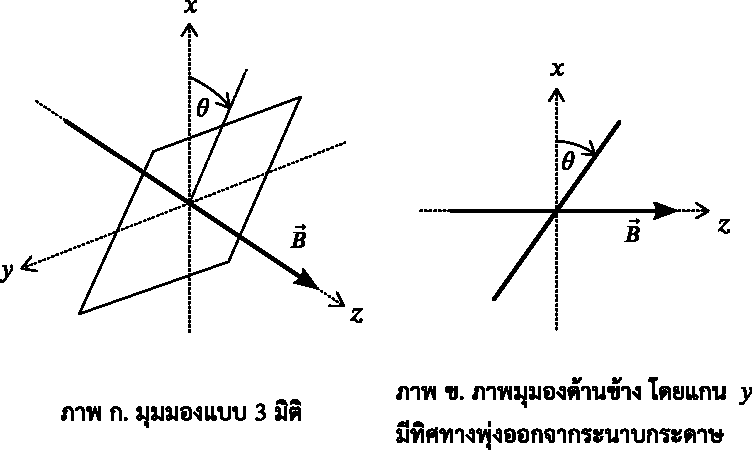
\includegraphics{images/12_21.pdf}
          \end{figure}
          ถ้าขณะมุม \(\theta=\SI{0}{\degree}\) ฟลักซ์แม่เหล็กที่ผ่านขดลวดเท่ากับ \(0.40\) เวเบอร์ สนามแม่เหล็กมีขนาดกี่เทสลาและเมื่อ \(\theta\) เพิ่มขึ้นจาก \(0\) องศา ถึง \(90\) องศา ฟลักซ์แม่เหล็กมีการเปลี่ยนแปลงอย่างไร
          \begin{figure}[H]
              \centering
              \begin{tabular}{c|c|c|}
                  \cline{2-3}
                     & ขนาดสนามแม่เหล็ก (เทสลา) & การเปลี่ยนแปลงฟลักซ์แม่เหล็ก \\
                  \cline{2-3}
                  1. & 0.20                   & น้อยลง                  \\
                  \cline{2-3}
                  2. & 0.80                   & มากขึ้น                  \\
                  \cline{2-3}
                  3. & 0.80                   & น้อยลง                  \\
                  \cline{2-3}
                  4. & 1.25                   & มากขึ้น                  \\
                  \cline{2-3}
                  5. & 1.25                   & น้อยลง                  \\
                  \cline{2-3}
              \end{tabular}
          \end{figure}
          \newpage
    \item นักเรียนคนหนึ่งมีแผ่นโพลารอยด์ที่ทราบแนวโพลาไรส์ 1 แผ่น และแหล่งกำเนิดแสงโพลาไรส์ที่ไม่ทราบแนวโพลาไรส์ เขาจึงคิดวิธีการทดลองเพื่อหาแนวโพลาไรส์ของแสงดังกล่าว ดังนี้ \\
          “ฉายแสงให้เคลื่อนที่ในทิศ \(+z\) ผ่านแผ่นโพลารอยด์ซึ่งอยู่ในแนวขนานกับระนาบ \(xy\) ดังภาพ แล้วสังเกตความสว่างของแสงในขณะที่หมุนแผ่นโพลารอยด์รอบแกน \(z\) อย่างช้า ๆ เพื่อหาตำแหน่งมุมที่ทำให้มองเห็นแสงมีความสว่างมากที่สุด” \\
          \begin{figure}[H]
              \centering
              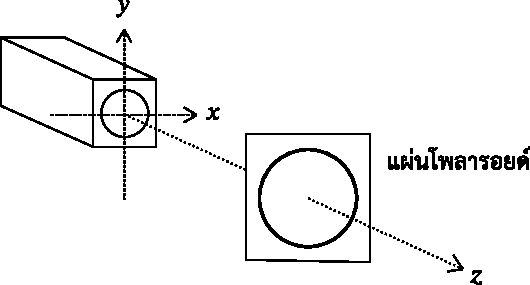
\includegraphics{images/13_22.pdf}
          \end{figure}
          วิธีข้างต้นจะสามารถใช้หาแนวโพลาไรส์ของแสงได้หรือไม่ เพราะเหตุใด
          \begin{enumerate}
              \item ไม่ได้ เพราะความสว่างของแสงที่ผ่านแผ่นโพลารอยด์จะคงที่ ไม่มีการเปลี่ยนแปลง
              \item ไม่ได้ เพราะการใช้แผ่นโพลารอยด์เพียงแผ่นเดียวจะไม่สามารถหาแนวโพลาไรส์ของแสงได้
              \item ไม่ได้ เพราะแสงโพลาไรส์จะมีสนามไฟฟ้าอยู่ในหลายแนวจึงไม่สามารถหาแนวโพลาไรส์ได้
              \item ได้ เพราะขณะที่แสงมีความสว่างมากที่สุด จะระบุได้ว่า แนวโพลาไรส์ของแสงอยู่ในแนวขนานกับแนวโพลาไรส์ของแผ่นโพลารอยด์
              \item ได้ เพราะขณะที่แสงมีความสว่างมากที่สุด จะระบุได้ว่า แนวโพลาไรส์ของแสงอยู่ในแนวตั้งฉากกับแนวโพลาไรส์ของแผ่นโพลารอยด์
          \end{enumerate}
          \newpage
    \item เมื่อฉายแสงความถี่ \(f\) ค่าต่าง ๆ ตกกระทบผิวโลหะชนิดหนึ่ง ได้ความสัมพันธ์ระหว่างความต่างศักย์หยุดยั้งกับความถี่ของแสง ดังกราฟ \\
          \begin{figure}[H]
              \centering
              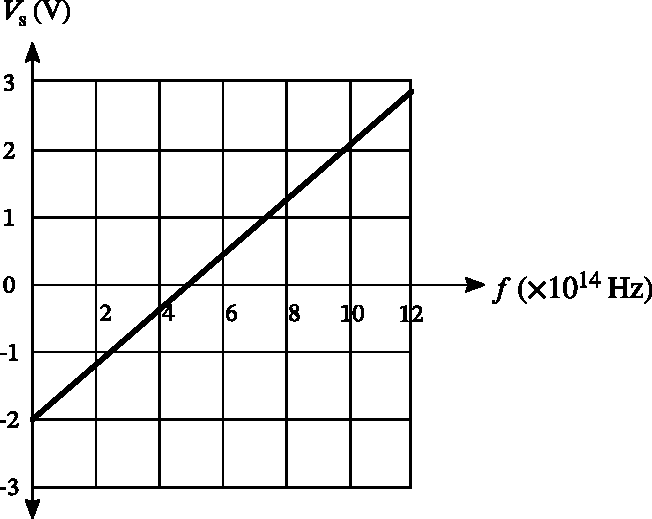
\includegraphics{images/17_23.pdf}
          \end{figure}
          กำหนดให้ \(e\) เป็นค่าประจุของอิเล็กตรอน \\
          \(h\) เป็นค่าคงตัวของพลังค์ ในหน่วยจูล วินาที \\
          ที่ความถี่ \(f\) พลังงานจลน์สูงสุดของโฟโตอิเล็กตรอนมีค่ากี่อิเล็กตรอนโวลต์
          \begin{enumerate}
              \item \(\dfrac{hf}{e}-2.0\)
              \item \(\dfrac{hf}{e}+2.0\)
              \item \(\dfrac{hf}{e}+5.0\)
              \item \(hf-2.0e\)
              \item \(hf+2.0e\)
          \end{enumerate}
          \newpage
    \item ปฏิกิริยานิวเคลียร์หนึ่ง เขียนแทนได้ด้วยสมการ \\
          \begin{equation*}
              \ch{^{16}_8O + ^{16}_8O -> ^{28}_{14}Si + ^4_2He}
          \end{equation*}
          \begin{tabular}{rl}
              กำหนดให้ & มวล \SI1 u เทียบเท่ากับพลังงาน \(932\) เมกะอิเล็กตรอนโวลต์       \\
                     & \(m_\text{O}\) เป็นมวลของออกซิเจนในหน่วย u                   \\
                     & \(m_\text{He}\) เป็นมวลของฮีเลียมในหน่วย u                    \\
                     & \(E\) เป็นพลังงานที่ได้จากปฏิกิริยานิวเคลียร์นี้ในหน่วยเมกะอิเล็กตรอนโวลต์
          \end{tabular} \\
          ปฏิกิริยานิวเคลียร์นี้ เป็นปฏิกิริยานิวเคลียร์ชนิดใด และ มวลในหน่วย u ของซิลิคอนมีค่าเท่าใด
          \begin{enumerate}
              \item ฟิชชัน และ \(2m_\text{O}+m_\text{He}-932E\)
              \item ฟิชชัน และ \(2m_\text{O}-m_\text{He}-\dfrac{E}{932}\)
              \item ฟิชชัน และ \(2m_\text{O}-m_\text{He}-932E\)
              \item ฟิวชัน และ \(2m_\text{O}-m_\text{He}-\dfrac{E}{932}\)
              \item ฟิวชัน และ \(2m_\text{O}-m_\text{He}-932E\)
          \end{enumerate}
    \item ในปรากฏการณ์หนึ่ง อนุภาค A เคลื่อนที่มาพบอนุภาค B แล้วทำให้ได้รังสีแกมมา ดังสมการ
          \begin{equation*}
              \ch{\text{อนุภาค\,A} + \text{อนุภาค\,B} -> \text{รังสีแกมมา}}
          \end{equation*}
          โดยที่อนุภาค A และ B เป็นอนุภาคที่ประกอบด้วย ควาร์กและแอนติควาร์ก \\
          พิจารณาข้อความต่อไปนี้
          \begin{itemize}
              \item[ก.] อนุภาค A และ อนุภาค B มีขนาดของประจุไฟฟ้าเท่ากัน
              \item[ข.] อนุภาคมูลฐานในอนุภาค B ยึดเหนี่ยวกันด้วยการแลกเปลี่ยนกลูออนระหว่างกัน
              \item[ค.] ผลรวมมวลของอนุภาค A กับอนุภาค B เท่ากับ มวลของโฟตอนของรังสีแกมมาโฟตอนเดียว
          \end{itemize}
          ข้อความใดถูกต้อง
          \begin{enumerate}
              \item ก. เท่านั้น
              \item ข. เท่านั้น
              \item ก. และ ข.
              \item ก. และ ค.
              \item ข. และ ค.
          \end{enumerate}
          \newpage
    \item วางวัตถุไว้หน้ากระจกโค้ง ซึ่งมีรัศมีความโค้ง \(28\) เซนติเมตร พบว่า เกิดภาพจริงขนาดเป็น \(2\) เท่าของวัตถุ วัตถุอยู่ห่างจากกระจกโค้งกี่\underline{เซนติเมตร}
          \vspace*{2cm}
    \item ออกแรงทิศทางขนานกับพื้นกระทำต่อวัตถุให้เคลื่อนที่ไปบนพื้นระดับเป็นระยะทาง \(30\) เมตร ความสัมพันธ์ระหว่างแรงกับตำแหน่งของวัตถุชิ้นนี้เป็นดังกราฟ \\
          \begin{figure}[H]
              \centering
              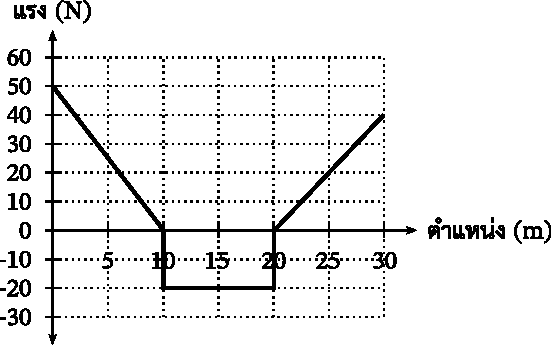
\includegraphics{images/30_27.pdf}
          \end{figure}
          ถ้าแรงนี้กระทำต่อวัตถุเป็นเวลา \(10\) วินาที กำลังเฉลี่ยของแรงนี้มีค่ากี่\underline{วัตต์}\
          \vspace*{2cm}
    \item แก๊สอุดมคติบรรจุอยู่ในภาชนะปิดปริมาตรคงตัว 0.5 ลูกบาศก์เมตร วัดความดันของแก๊สขณะที่แก๊สมีอุณหภูมิค่าต่าง ๆ แล้วนำข้อมูลที่วัดได้ไปเขียนกราฟแสดงความสัมพันธ์ระหว่างความดันของแก๊สและอุณหภูมิของแก๊ส ได้ผลดังกราฟ \\
          \begin{figure}[H]
              \begin{minipage}[ht]{0.5\linewidth}
                  กำหนดให้ \\
                  ค่าคงตัวแก๊ส \(R = \SI{8.3}{J/(mol\,K)}\) \\
                  ค่าคงตัวอาโวกาโดร \(N_\text{A} = \SI{6.0e23}{mol^{-1}}\) \\
                  ค่าคงตัวโบลต์ซมันน์ \(k_\text{B} = \SI{1.4e-23}{J/K}\) \\
                  แก๊สภายในภาชนะมีจำนวนกี่\underline{โมล}
              \end{minipage}
              \begin{minipage}[ht]{0.5\linewidth}
                  \begin{figure}[H]
                      \raggedright
                      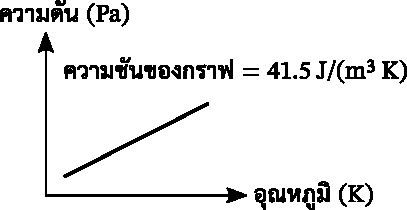
\includegraphics{images/28_28.pdf}
                  \end{figure}
              \end{minipage}
          \end{figure}
          \vspace*{2cm}
    \item วัตถุเคลื่อนที่ในแนวตรงโดยเริ่มจากหยุดนิ่ง ซึ่งความเร็ว ณ เวลาต่าง ๆ แสดงได้ดังกราฟ \\
          \begin{figure}[H]
              \centering
              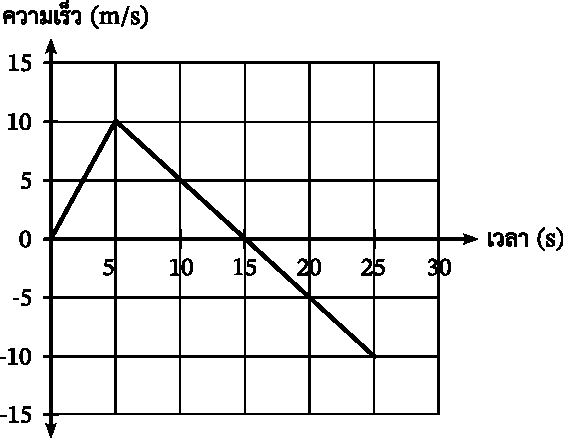
\includegraphics{images/29_29.pdf}
          \end{figure}
          ความเร่งเฉลี่ยของวัตถุนี้ ในช่วงเวลา \(t = \SI{5}{s}\) ถึง \(t = \SI{25}{s}\) มีขนาดกี่\underline{เมตรต่อวินาที\(^2\)}
          \vspace*{2cm}
    \item ต่อตัวต้านทาน \(R\) ที่มีความต้านทาน \(10\) โอห์ม กับลวดตัวนำ X และ Y ที่วางขนานกันและอยู่ห่างกันเป็นระยะ \(25\) เซนติเมตร แล้ววางแท่งตัวนำ Z ตั้งฉากกับลวดตัวนำทั้งสอง ดังภาพ ซึ่งเป็นมุมมองจากด้านบน \\
          จากนั้น ดึงแท่งตัวนำ Z ให้เคลื่อนที่ไปทางขวาด้วยความเร็วคงตัว \(40\) เซนติเมตรต่อวินาที ในบริเวณที่มีสนามแม่เหล็กสม่ำเสมอ \(1\) เทสลา ซึ่งมีทิศพุ่งออกและตั้งฉากกับระนาบกระดาษ \\
          กำหนดให้ ความต้านทานของลวดตัวนำ X และ Y และแท่งตัวนำ Z มีค่าน้อยมากเมื่อเปรียบเทียบกับของตัวต้านทาน \(R\) \\
          \begin{figure}[H]
              \centering
              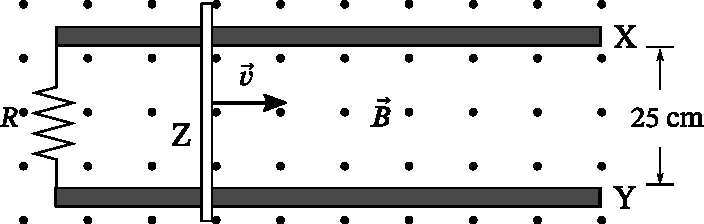
\includegraphics{images/27_30.pdf}
          \end{figure}
          กระแสไฟฟ้าเหนี่ยวนำที่ผ่านตัวต้านทานมีค่ากี่\underline{แอมแปร์}
          \vspace*{2cm}
\end{enumerate}
\newpage
\begin{center}
    \huge{\textbf{เฉลย}}
\end{center}
\begin{enumerate}
    \item 3. 58 และ 4. 58.4 \footnote{ข้อสอบมีความผิดพลาด แต่ในทางปฏิบัติข้อ 3 เป็นข้อที่ถูกต้องมากกว่า}
    \item 5. 60
    \item 3. อัตราเร็วเชิงมุมของ \(m_1\) มีค่าเท่ากับอัตราเร็วเชิงมุมของ \(m_2\)
    \item 5. ข. และ ค.
    \item 1. \(\dfrac{u^2}{2\mu_s g}\)
    \item 2. \(mg\cos\theta\)
    \item 1. \(I_1\) มากกว่า \(I_2\) เพราะพื้นที่ใต้กราฟของครั้งที่ 1 มากกว่าครั้งที่ 2
    \item 4. 0.5
    \item 1. \hfill
          \begin{figure}[H]
              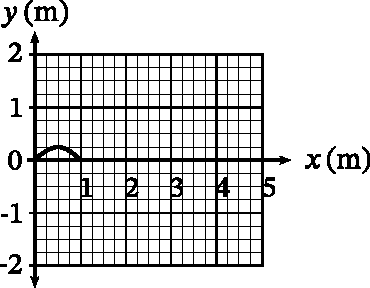
\includegraphics{images/21_9_1.pdf}
          \end{figure}
    \item 3. \(\num{1.5e2}\)
    \item 3. ส้อมเสียง C และ 10 ครั้ง
    \item 2. \(\num{1.5e8}\) เมตรต่อวินาที และ แสงจะหักเหออกสู่อากาศด้วยมุมหักเหที่มากกว่า \(20\) องศา
    \item 4. ก. และ ค.
    \item 2. ลวดโลหะ A และ \num{5.0e10} พาสคัล
    \item 2. \(38R\) และ ปริมาตรลดลง
    \item 5. \num{9.8e-2}
    \item 5. ชนิดต่างกัน, \(Q\sqrt{\dfrac{nk}{Mg}}\)
    \item 5. ลง, A มากกว่า B, A มากกว่า B
    \item 2. 300
    \item 1. ก. เท่านั้น
    \item 3. 0.80, น้อยลง
    \item 4. ได้ เพราะขณะที่แสงมีความสว่างมากที่สุด จะระบุได้ว่า แนวโพลาไรส์ของแสงอยู่ในแนวขนานกับแนวโพลาไรส์ของแผ่นโพลารอยด์
    \item 1. \(\dfrac{hf}{e}-2.0\)
    \item 4. ฟิวชัน และ \(2m_\text{O}-m_\text{He}-\dfrac{E}{932}\)
    \item 3. ก. และ ข.
    \item \SI{21}{cm}
    \item \SI{25}{W}
    \item \SI{2.5}{mol}
    \item \SI{1}{m/s^2}
    \item \SI{0.01}{A}
\end{enumerate}
\end{document}